\documentclass[11pt,a4paper]{article}
\usepackage[T1]{fontenc}
\usepackage[utf8]{inputenc}
\IfFileExists{brazil.ldf}{\usepackage[brazil]{babel}}{\renewcommand{\abstractname}{Resumo}\renewcommand{\refname}{Referências}}
\usepackage[margin=2.1cm]{geometry}
\usepackage{lmodern,microtype,amsmath,amssymb,booktabs,tabularx,graphicx,float,xcolor}
\usepackage[hidelinks]{hyperref}
\usepackage{fancyhdr}
\pagestyle{fancy}\fancyhf{}\fancyhead[L]{\small MO438 -- Redes Complexas}\fancyhead[R]{\small Relatório final -- 20/11/2026}\fancyfoot[C]{\thepage}
\setlength{\headheight}{14pt}\setlength{\parindent}{1.1em}\setlength{\parskip}{3pt}
\renewcommand{\arraystretch}{1.14}
\newcommand{\figura}[3]{\begin{figure}[H]\centering\includegraphics[width=\linewidth,height=#2,keepaspectratio]{figuras/#1.pdf}\caption{#3}\end{figure}}
\begin{document}
\begin{center}
\noindent\begin{minipage}[c]{.68\linewidth}
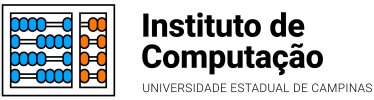
\includegraphics[width=5.8cm]{identidade/logo_ic.png}
\end{minipage}\hfill
\begin{minipage}[c]{.28\linewidth}\raggedleft

\includegraphics[width=2.5cm]{identidade/logo_unicamp.jpg}
\end{minipage}\par
\vspace{5pt}
{\Large\bfseries Estrutura do debate midiático sobre inteligência artificial: análise comparativa e temporal de redes de entidades}\par
\vspace{7pt}
Pedro Henrique de Carvalho Godoy\par
{\small Disciplina MO438 -- Redes Complexas | Professor: Ruben Interian}
\end{center}
\begin{abstract}
O objetivo geral é analisar comparativamente e ao longo do tempo redes de entidades extraídas de notícias sobre inteligência artificial de diferentes fontes jornalísticas, utilizando a caracterização global como referência. O estudo combina a rede global dos períodos disponíveis, a comparação de G1, Folha de S.Paulo e CNN Brasil em 2025 e 32 cortes anuais acumulados da Folha, de 1994 a 2025. Das 23.657 notícias selecionadas, 9.113 sustentam a rede global, com 40.627 entidades e 57.536 pares simples. A estrutura é esparsa e heterogênea, com uma componente dominante e numerosas componentes pequenas. As fontes compartilham entidades centrais, mas apresentam baixa sobreposição de pares. A visibilidade documental é concentrada: aproximadamente 1\% das entidades reúne 35,07\% das aparições entidade--notícia. A análise temporal distingue crescimento, formação de conexões, reforço de vínculos e mudanças de protagonismo. Há associação positiva entre grau anterior e novos vizinhos nas transições com variação. Os resultados descrevem a rede observada, condicionada às lacunas de extração, sem demonstrar causalidade ou um mecanismo gerador livre de escala.
\end{abstract}
\section{Introdução e objetivos}
A cobertura jornalística registra entidades, acontecimentos e relações envolvendo o desenvolvimento e os usos da inteligência artificial (IA). Representá-la como rede permite examinar quais entidades se conectam, quais posições ocupam e como a estrutura observada varia entre fontes e períodos. A rede descreve o noticiário coletado; não mede diretamente a opinião pública nem a totalidade das relações sociais sobre IA.

O trabalho deriva da dissertação do autor~\cite{godoy2026}, que estabeleceu a integração entre coleta de notícias, reconhecimento de entidades, extração de relações, resolução de menções e análise em rede. A contribuição desta disciplina concentra-se na comparação e na dimensão temporal, aprofundando a caracterização estrutural. Os resultados finais utilizam a base consolidada desta edição.

\paragraph{Objetivo geral.} Analisar comparativamente e ao longo do tempo redes de entidades extraídas de notícias sobre IA de diferentes fontes jornalísticas, utilizando a caracterização global como referência.

\paragraph{Síntese da entrega parcial.} A análise inicial apresentou o projeto e sua estratégia de extração de entidades e relações, caracterizando uma rede global com 54.256 vértices e 84.846 pares simples. O grau médio de 3,128 e a baixa densidade indicavam uma estrutura esparsa. A entrega final amplia essa análise com comparação entre fontes, comunidades, centralidades e evolução temporal. A base e a consolidação foram revistas; diferenças de tamanho entre as edições refletem essas mudanças e não representam redução histórica do debate.

\paragraph{Objetivos específicos.} (i) Caracterizar conectividade, fragmentação, distâncias e heterogeneidade da rede global; (ii) comparar estrutura, entidades centrais e comunidades entre fontes no período comum de 2025; (iii) examinar a evolução acumulada da Folha, distinguindo crescimento, formação e reforço de conexões; (iv) investigar persistência dos destaques, distribuição de graus e associação entre conectividade anterior e ganhos; (v) preservar a ligação dos resultados às notícias e explicitar o efeito da cobertura.

\clearpage
\section{Dados e metodologia}
\subsection{Corpus e delimitações da edição}
A base selecionada contém 23.657 notícias de G1, Folha de S.Paulo e CNN Brasil, de 1994 a 2026. Dessas, 9.113 fornecem relações para a rede global desta edição. Aqui, \textbf{global} significa reunir as três fontes e todos os períodos com relações disponíveis; não significa cobertura integral do acervo nem de toda a produção jornalística. As relações efetivamente incorporadas vão de 1994 a 2025. A caracterização global não se restringe a 2025: 6.511 notícias de suporte são desse ano e 2.602 são de outros anos. A participação de 2025, de 71,45\%, deve ser considerada ao interpretar os resultados globais.

A comparação entre fontes utiliza o ano de 2025, com 7.615 notícias selecionadas. A análise temporal considera a Folha, com 10.717 notícias selecionadas e 5.250 notícias que fornecem relações. São 32 cortes anuais acumulados, de 1994 a 2025, abrangendo os 19 marcos da entrega parcial. Um corte em $t$ reúne as relações das notícias desde 1994 até $t$. A série tem lacunas de processamento: em 2021, nenhuma notícia teve RE concluída; outros anos têm cobertura parcial. Assim, existir um corte anual não significa que todas as notícias daquele ano tenham sido processadas.

\subsection{Entidades, relações e representações}
O reconhecimento de entidades nomeadas (NER) identifica pessoas, organizações e locais; a extração de relações (RE) identifica vínculos semânticos entre essas entidades. A resolução de entidades reúne menções consideradas equivalentes sob um mesmo identificador. A entrega parcial descreve essa etapa com referência às representações multilíngues E5~\cite{wang2024e5}; esta análise utiliza os identificadores do registro já consolidado. Essa identificação usa o conjunto completo de notícias e é aplicada também aos anos anteriores. Portanto, a série acompanha as entidades identificadas hoje, sem reconstruir como elas poderiam ser reconhecidas apenas com as informações de cada época.

A rede semântica preserva direção e tipo da relação. O peso de uma aresta conta registros extraídos para a mesma combinação de entidades, direção e tipo: três registros resultam em peso 3, sem garantir três notícias ou fatos independentes. Excluindo identidade, autolaços e os grupos cadastrados das fontes, restam 181.348 registros e 83.188 arestas dirigidas e tipadas.

A projeção simples não dirigida associa um único vínculo a cada par conectado, independentemente de direção, rótulo ou peso. Para comunidades, utiliza-se uma projeção ponderada não dirigida: somam-se os pesos das relações entre cada par, em ambas as direções. Os nós são entidades participantes de relações retidas; a ausência de isolados decorre desse critério de inclusão e não constitui um achado independente sobre a integração do debate.

\subsection{Indicadores e verificações}
A caracterização e a interpretação estrutural utilizam os conceitos de redes complexas apresentados nos materiais da disciplina MO438~\cite{interian2026mo438}.
Na projeção simples, $k_i$ conta vizinhos distintos, $\langle k\rangle=2M/N$ e $\rho=2M/[N(N-1)]$. Reportam-se a média de clusterização local para $k_i\geq2$ e a transitividade $3T/\sum_i\binom{k_i}{2}$, além de componentes e distâncias em número de arestas. A distância média, o diâmetro e o raio referem-se à maior componente conexa (GCC).

O grau conta vizinhos distintos; a força soma os pesos de todas as relações incidentes; e o PageRank ponderado considera a estrutura dos vínculos recebidos na rede dirigida, com amortecimento 0,85. Para comparar participações no PageRank, divide-se cada escore pela soma dos escores. Essa normalização não o transforma em uma probabilidade de circulação de informação. Como a rede combina tipos diferentes de relação, centralidade exige interpretação e não mede diretamente poder ou influência social.

Contagens, pesos, distâncias, escores e conectividade das comunidades foram conferidos por procedimentos independentes, sem substituir a avaliação dos erros de NER, RE e resolução.

\clearpage
\section{Caracterização estrutural global, de 1994 a 2025}
A rede global analítica reúne 40.627 entidades e 57.536 pares simples. Sua GCC contém 32.575 entidades, equivalentes a 80,18\% dos nós. As outras componentes são importantes para a descrição da fragmentação, embora representem uma parcela menor das entidades. A Tabela~\ref{tab:global} distingue contagens da rede completa e métricas restritas à GCC.

\begin{table}[H]\centering\small
\caption{Rede global dos períodos disponíveis, de 1994 a 2025. Distâncias são exatas na GCC.}\label{tab:global}
\begin{tabularx}{\linewidth}{XrXr}\toprule
Indicador & Valor & Indicador & Valor\\\midrule
Entidades & 40.627 & Pares simples & 57.536\\
Arestas dirigidas e tipadas & 83.188 & Ocorrências retidas & 181.348\\
Grau médio & 2,8324 & Densidade & $6,9719\times10^{-5}$\\
Grau mínimo / máximo & 1 / 1.796 & Mediana do grau & 1\\
Nós com grau 1 & 23.080 & Nós com grau até 2 & 31.925\\
Clusterização ($k\geq2$) & 0,2436 & Transitividade & 0,0099\\
Componentes conexas & 3.259 & Nós na GCC & 32.575\\
Distância média (GCC) & 4,8596 & Diâmetro / raio (GCC) & 20 / 10\\\bottomrule
\end{tabularx}
\end{table}

O grau médio baixo e a densidade pequena descrevem uma rede esparsa. A maior parte das entidades possui poucos vizinhos, coexistindo com um conjunto reduzido de entidades de conectividade elevada. A CCDF da Figura~\ref{fig:global} representa $P(K\geq k)$ e torna essa heterogeneidade visível, sem constituir, por si só, teste de lei de potência.

\begin{figure}[H]\centering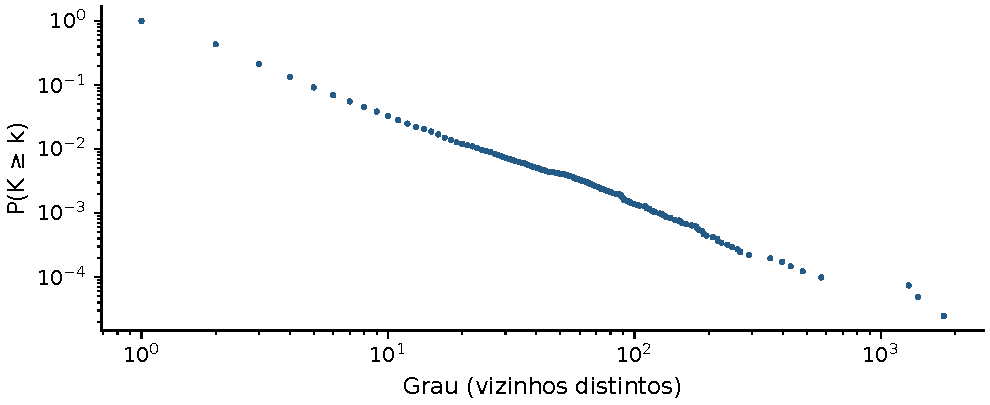
\includegraphics[width=.86\linewidth,height=6.5cm,keepaspectratio]{figuras/global_ccdf.pdf}\caption{Distribuição acumulada complementar dos graus da projeção simples global. Os eixos logarítmicos não demonstram uma classe geradora de redes.}\label{fig:global}\end{figure}

A clusterização média entre nós elegíveis é muito maior que a transitividade. As duas medidas ponderam a estrutura de maneiras diferentes: a primeira atribui o mesmo peso a cada nó elegível, enquanto a segunda depende da quantidade de triplas. Portanto, a diferença é compatível com heterogeneidade no fechamento triádico e não constitui inconsistência aritmética.

As distâncias foram calculadas exatamente entre os nós da GCC. O diâmetro 20 e a média 4,8596 descrevem caminhos entre entidades na rede de relações extraídas. A rede completa é desconexa; por isso, não se informa um diâmetro global finito. Tampouco se deduzem velocidade de circulação de informação ou propriedades de mundo pequeno apenas dessas distâncias.

\clearpage
\section{Entidades centrais e concentração de visibilidade}
\subsection{Centralidade e presença nas notícias}
Os seis líderes por grau global estão na Tabela~\ref{tab:lideres}. Brasil ocupa o primeiro lugar em quantidade de vizinhos, enquanto Estados Unidos participa de mais notícias da rede. As cinco primeiras posições de PageRank coincidem com as de grau; Google é o sexto por grau e o nono por PageRank. Há convergência no topo, mas as medidas descrevem aspectos diferentes do protagonismo.

\begin{table}[H]\centering\small
\caption{Seis líderes por grau global. Notícias e porcentagens referem-se à participação da entidade em relações nas 9.113 notícias que sustentam a rede.}\label{tab:lideres}
\begin{tabularx}{\linewidth}{Xrrrr}\toprule
Entidade & Grau & Força & Notícias & \% de notícias\\\midrule
Brasil & 1.796 & 11.030 & 1.775 & 19,48\\
Estados Unidos & 1.414 & 10.876 & 2.216 & 24,32\\
São Paulo & 1.295 & 5.082 & 1.055 & 11,58\\
China & 573 & 5.347 & 771 & 8,46\\
SP & 481 & 2.326 & 392 & 4,30\\
Google & 430 & 3.769 & 650 & 7,13\\
\bottomrule\end{tabularx}\end{table}

Para medir \textbf{visibilidade documental}, conta-se uma vez cada entidade em cada notícia na qual ela participa de relações incorporadas à rede. Uma entidade com várias relações na mesma notícia continua contando uma única vez. A medida se refere à participação na rede extraída; menções sem relação incorporada ficam fora desse indicador. Uma notícia pode contribuir para várias entidades, de modo que as porcentagens da tabela não devem ser somadas.

No conjunto global, há 102.807 aparições entidade--notícia. Ordenadas por essa visibilidade, as 407 entidades mais presentes (aproximadamente 1\% dos nós) concentram 35,07\% das aparições; as 2.032 primeiras (aproximadamente 5\%), 50,41\%; e as 4.063 primeiras (aproximadamente 10\%), 57,82\%. O Gini é 0,5670. Essas participações usam o total de aparições, não o número de notícias, e mostram concentração da presença relacional em um subconjunto das entidades.

\figura{visibilidade}{5.3cm}{Curva de Lorenz da visibilidade documental global. A distância em relação à diagonal indica desigualdade na distribuição das aparições entidade--notícia.}

A concentração de visibilidade é distinta da concentração de grau: a primeira descreve presença documental; a segunda, diversidade de vizinhos. Nenhuma delas, isoladamente, mede espaço de texto, destaque editorial ou avaliação positiva de uma entidade.

\clearpage
\subsection{Seis exemplos de protagonismo por tipo}
Para interpretar o resultado sem restringi-lo aos lugares que dominam o ranking geral, selecionam-se as duas entidades de maior grau em cada tipo: local, organização e pessoa. Empates são resolvidos pelo identificador. Trata-se de uma seleção descritiva por critério explícito, não de uma amostra representativa das entidades. A Tabela~\ref{tab:casos} apresenta os seis casos.

\begin{table}[H]\centering\small
\caption{Dois líderes por grau em cada tipo. A visibilidade é calculada sobre as mesmas 9.113 notícias da rede global.}\label{tab:casos}
\begin{tabularx}{\linewidth}{Xrrrr}\toprule
Entidade & Grau & Força & Notícias & \% de notícias\\\midrule
Brasil & 1.796 & 11.030 & 1.775 & 19,48\\
Estados Unidos & 1.414 & 10.876 & 2.216 & 24,32\\
Google & 430 & 3.769 & 650 & 7,13\\
Univ. de São Paulo & 356 & 1.029 & 273 & 3,00\\
Donald Trump & 249 & 3.109 & 825 & 9,05\\
Luiz Inácio Lula da Silva & 151 & 1.247 & 380 & 4,17\\
\bottomrule\end{tabularx}\end{table}

\paragraph{Brasil.} Com 1.796 vizinhos e presença relacional em 1.775 notícias, lidera a diversidade de conexões. Entre seus pares de maior peso estão São Paulo (760 registros), América Latina (528) e Rio de Janeiro (238). Relações classificadas como inclusão somam 7.569 dos 11.030 registros incidentes. Sua posição central depende, em parte, da maneira como referências territoriais conectam outras entidades.

\paragraph{Estados Unidos.} Tem menos vizinhos que Brasil, mas participa de mais notícias: 2.216, ou 24,32\% do total da rede. Seu par de maior peso é Donald Trump (1.593 registros), seguido de Washington (342) e TikTok (298). O contraste com Brasil mostra que maior presença documental não implica maior diversidade de vizinhos.

\paragraph{Google.} Lidera o grau entre organizações, com 430 vizinhos e 650 notícias. Seus pares de maior peso são Chrome (750), Alphabet (571) e YouTube (180). A força de 3.769 indica recorrência de relações que o grau, ao contar cada vizinho apenas uma vez, não representa.

\paragraph{Universidade de São Paulo.} É a segunda organização por grau, com 356 vizinhos e 273 notícias. Em comparação com Google, apresenta grau relativamente próximo, mas força e presença documental menores. Ribeirão Preto (40), São Paulo (37) e São Carlos (31) são os pares de maior peso. O caso evidencia diversidade de conexões sem recorrência tão elevada.

\paragraph{Donald Trump.} Lidera o grau entre pessoas, com 249 vizinhos, força 3.109 e participação em 825 notícias. Embora tenha menos vizinhos que Google, aparece em mais notícias. O peso de seu par com Estados Unidos, 1.593, corresponde a aproximadamente metade de sua força. O protagonismo combina, portanto, presença documental e recorrência concentrada nesse par.

\paragraph{Luiz Inácio Lula da Silva.} É o segundo por grau entre pessoas, com 151 vizinhos e participação em 380 notícias. Os pares com PT (555), Brasil (188) e governo Lula (48) estão entre os mais recorrentes. A força de 1.247, diante do grau menor, reforça a distinção entre multiplicidade de vizinhos e repetição de vínculos.

Os pesos citados somam os tipos e as direções das relações em cada par; não equivalem a notícias ou fatos independentes. Os exemplos descrevem os dados extraídos, sem atribuir influência causal às entidades. São Paulo e SP continuam associados a identificadores separados: sua eventual equivalência exige revisão contextual e não é presumida nesta análise.

\clearpage
\section{Comunidades globais}
\subsection{Partições e sensibilidade}
Louvain~\cite{blondel2008} e Leiden~\cite{traag2019} foram aplicados à projeção ponderada não dirigida, com resolução $\gamma=1$. Louvain é a referência do pipeline; Leiden usa sementes 42, 43 e 44, sendo a primeira a referência visual previamente definida. A modularidade é recalculada sobre as partições retornadas:
\[
Q=\sum_c\left[\frac{W_c}{W}-\left(\frac{S_c}{2W}\right)^2\right],
\]
em que $W_c$ conta o peso interno de cada par uma vez e $S_c$ soma as forças dos nós da comunidade. Os resultados não representam uma busca exaustiva por resoluções ou soluções.

\begin{table}[H]\centering\small
\caption{Partições globais e diagnóstico de conectividade interna.}\label{tab:comunidades}
\begin{tabular}{lrrrr}\toprule
Execução & Comunidades & $Q$ & Maior grupo & Grupos desconexos\\\midrule
Louvain & 3.407 & 0,797902 & 3.480 & 12\\
Leiden, semente 42 & 3.517 & 0,791399 & 5.032 & 0\\
Leiden, semente 43 & 3.539 & 0,790834 & 5.323 & 0\\
Leiden, semente 44 & 3.541 & 0,791042 & 5.337 & 1\\\bottomrule
\end{tabular}
\end{table}

Entre Louvain e Leiden 42, o ARI é 0,6172 e a NMI é 0,8781 na rede inteira. Restritas aos nós da GCC, as partições globais têm ARI 0,6101 e NMI 0,7916; não houve nova detecção exclusiva na GCC. A concordância maior na rede completa pode refletir o acordo nas numerosas componentes pequenas. A modularidade de agrupar apenas pelas componentes é 0,0885, uma referência descritiva para a fragmentação, não uma parcela aditiva a subtrair universalmente de $Q$.

\paragraph{Diagnóstico de conectividade.} A execução Leiden 44 contém uma comunidade com 46 entidades, separada em dois grupos de 14 e 32 nós. A projeção completa foi conferida e quatro execuções diagnósticas no Neo4j GDS 2026.09.0 reproduziram exatamente a mesma partição, inclusive ao alterar a renumeração dos grupos, ampliar o número de níveis e reduzir a tolerância. O resultado é reproduzível nessas condições, mas sua causa não foi estabelecida. Preservam-se as partições, com Louvain como referência e Leiden 42 como comparação previamente definida. Conectividade também não comprova coerência temática: essa interpretação requer leitura das relações e notícias.

\clearpage
\section{Comparação entre fontes em 2025}
\subsection{Cobertura e estrutura}
A comparação mantém o mesmo ano e os mesmos critérios de construção. Entretanto, as fontes têm volumes e coberturas distintos, conforme a Tabela~\ref{tab:fontes}. A cobertura de RE integral é 90,32\% na CNN Brasil, 90,95\% na Folha e 94,09\% no G1. As medidas descrevem as redes observadas e não isolam um efeito editorial de diferenças de coleta ou processamento.

\begin{table}[H]\centering\small
\caption{Redes por fonte no ano de 2025. $C$ é a média local para $k\geq2$.}\label{tab:fontes}
\begin{tabularx}{\linewidth}{Xrrr}\toprule
Indicador & CNN Brasil & Folha & G1\\\midrule
Notícias selecionadas & 2.087 & 3.413 & 2.115\\
RE integralmente concluída & 1.885 & 3.104 & 1.990\\
Notícias que sustentam a rede & 1.750 & 2.887 & 1.874\\
Entidades & 6.517 & 15.567 & 11.578\\
Pares simples & 8.203 & 20.601 & 15.132\\
Ocorrências retidas & 27.163 & 61.082 & 46.424\\
Grau médio & 2,5174 & 2,6468 & 2,6139\\
Densidade ($\times10^{-4}$) & 3,8634 & 1,7003 & 2,2579\\
$C$ & 0,2175 & 0,2243 & 0,2718\\
Transitividade & 0,0201 & 0,0133 & 0,0246\\
Nós na GCC (\%) & 69,77 & 74,82 & 76,86\\\bottomrule
\end{tabularx}
\end{table}

A Folha apresenta a maior rede em número de nós e pares, mas o G1 tem maiores clusterização e transitividade. A CNN Brasil apresenta a maior densidade, juntamente com a menor rede. Como a densidade depende do denominador $N(N-1)$, ela não pode ser lida isoladamente como maior integração substantiva. Os graus médios, próximos de 2,5--2,6, coexistem com diferentes tamanhos e participações da GCC.

\figura{sources_ccdf}{5.8cm}{CCDF dos graus por fonte em 2025, nas projeções simples. A comparação usa o mesmo período, mas não iguala o tamanho dos acervos ou a cobertura de extração.}

\subsection{Sobreposição e atores centrais}
O Jaccard dos conjuntos de entidades é 0,1197 entre CNN e Folha, 0,0949 entre CNN e G1 e 0,1014 entre Folha e G1. Para pares, os valores são menores: 0,0637, 0,0479 e 0,0499. Assim, compartilhar algumas entidades não implica compartilhar a maior parte de suas conexões. Tais valores também são sensíveis ao tamanho das redes, à cobertura e à resolução compartilhada.

\clearpage
\subsection{Rankings e comunidades por fonte}
Estados Unidos lidera o grau na CNN Brasil, com 376 vizinhos; Brasil lidera na Folha (854) e no G1 (431). Os quatro primeiros da CNN são Estados Unidos, Brasil, China e São Paulo. Na Folha, Brasil, Estados Unidos, São Paulo e China são seguidos por OpenAI. No G1, Brasil, Estados Unidos, São Paulo e SP são seguidos por Salvador. A presença de lugares no topo demanda examinar relações de localização e granularidade geográfica, sem equiparar centralidade a poder político ou tecnológico.

A sobreposição entre CNN e Folha entre os 20 primeiros por grau é de 16 entidades, correspondente a Jaccard 0,6667, enquanto a sobreposição entre todos os seus nós é 0,1197. A diferença mostra que um núcleo de entidades muito conectadas pode ser compartilhado, apesar da diversidade das entidades periféricas e dos pares. O ranking considera 20 entidades, com desempate por identificador.

\begin{table}[H]\centering\small
\caption{Partições por fonte: referência Louvain e Leiden com semente 42.}\label{tab:fontescom}
\begin{tabular}{llrrr}\toprule
Fonte & Execução & Comunidades & $Q$ & Grupos desconexos\\\midrule
CNN Brasil & Louvain & 791 & 0,823538 & 1\\
CNN Brasil & Leiden 42 & 801 & 0,824006 & 0\\
Folha & Louvain & 1.673 & 0,808427 & 4\\
Folha & Leiden 42 & 1.689 & 0,809171 & 2\\
G1 & Louvain & 1.081 & 0,856332 & 1\\
G1 & Leiden 42 & 1.095 & 0,855818 & 1\\\bottomrule
\end{tabular}
\end{table}

O G1 apresenta a maior modularidade entre as referências mostradas, mas comparar $Q$ entre redes diferentes não constitui um teste de organização editorial. Diferenças de tamanho, peso, fragmentação e composição interferem na medida. Também não se observa superioridade uniforme de uma implementação em todas as redes: a pontuação Louvain do G1 supera a Leiden 42, enquanto ocorre o inverso na CNN e na Folha.

A conferência das partições por fonte reproduziu as contagens de comunidades desconexas. A ocorrência também na Folha e no G1 limita qualquer afirmação de que todas as comunidades obtidas por Leiden sejam internamente conectadas. Os resultados são apresentados com esse diagnóstico; atribuir temas aos grupos exigiria validação qualitativa das notícias e relações.

A comparação final concentra-se nas três redes por fonte. A rede conjunta de 2025, citada no planejamento parcial, não foi incluída nesta edição; a rede global agrega os períodos disponíveis e funciona como referência geral, sem substituir esse recorte.

\clearpage
\section{Evolução temporal acumulada da Folha}
\subsection{Crescimento e cobertura}
A série cresce de 101 entidades e 85 pares em 1994 para 27.642 entidades, 37.099 pares e 103.966 ocorrências no corte acumulado de 2025. A GCC final contém 21.577 entidades (78,06\%); o grau médio final é 2,6842. O crescimento acumulado reflete tanto a incorporação de documentos como a formação de conexões observadas. O desenho garante persistência dos nós e pares já incorporados; portanto, não serve para medir seu desaparecimento.

\begin{table}[H]\centering\small
\caption{Cobertura anual de RE integral na Folha e nós acumulados selecionados.}\label{tab:cobertura}
\begin{tabular}{lrrrr}\toprule
Ano & Notícias do ano & RE integral & Cobertura (\%) & Nós acumulados\\\midrule
2019 & 412 & 399 & 96,84 & 11.793\\
2020 & 437 & 24 & 5,49 & 11.896\\
2021 & 399 & 0 & 0,00 & 11.896\\
2024 & 2.256 & 106 & 4,70 & 14.798\\
2025 & 3.413 & 3.104 & 90,95 & 27.642\\\bottomrule
\end{tabular}
\end{table}

A repetição de 11.896 nós em 2020 e 2021 decorre da ausência de relações retidas de 2021 nesta edição, não de estabilidade demonstrada na realidade. O salto de 2025 inclui 12.844 entidades vistas pela primeira vez na rede acumulada e coincide com cobertura muito superior à de 2024. Assim, sua magnitude não deve ser atribuída exclusivamente ao crescimento do debate sobre IA naquele ano.

\figura{temporal_growth}{7.0cm}{Entidades e pares acumulados na Folha (esquerda) e proporção anual de notícias com RE concluída (direita). A cobertura desigual condiciona a interpretação do crescimento.}

Os marcos de referência organizam a observação da série; não representam, por si, fronteiras históricas do desenvolvimento da IA. O detalhe anual amplia a análise, mas a interpretação continua condicionada à quantidade de notícias efetivamente processadas.

\clearpage
\subsection{Formação e reforço de conexões}
Depois do estoque inicial de 1994, as 31 transições anuais acrescentam 37.014 pares. A classificação utiliza a presença dos extremos na rede acumulada anterior, e não sua idade real ou existência fora do corpus.

\begin{table}[H]\centering
\caption{Pares novos depois de 1994, segundo a presença anterior de seus extremos.}\label{tab:formacao}
\begin{tabular}{lrr}\toprule
Classe & Pares & Participação (\%)\\\midrule
Nova--nova & 13.700 & 37,01\\
Antiga--nova & 18.611 & 50,28\\
Antiga--antiga & 4.703 & 12,71\\\bottomrule
\end{tabular}
\end{table}

A classe antiga--nova corresponde a aproximadamente metade dos pares acrescentados. Ela mostra que novas entidades frequentemente ingressam conectadas a entidades já presentes. Ainda assim, a composição não demonstra ligação preferencial: para isso, seria necessário examinar quais entidades anteriores recebem os vínculos e comparar mecanismos e oportunidades de ligação.

A recorrência permite distinguir formação e reforço. Depois de 1994, 80.218 registros de relações aparecem em pares novos e 23.548 acrescentam peso a pares já existentes. Assim, a expansão ocorre tanto pela criação de conexões quanto pela repetição de vínculos anteriormente observados.

\figura{connections}{5.5cm}{Composição dos 37.014 pares novos somados nas transições de 1994 a 2025. Nova e antiga indicam presença na rede do corte anterior. A agregação dá maior peso aos anos com mais pares observados.}

\subsection{Persistência dos destaques}
Na transição 2024--2025, 15 das 20 entidades do ranking anterior permanecem entre as 20 primeiras: retenção de 75\% e Jaccard 0,60. Cinco entram e cinco deixam essa seleção. A entrada ou saída do ranking não corresponde necessariamente à entrada ou saída da rede, e a persistência acumulada não mede presença jornalística contínua.

A retenção de 100\% em 2020--2021 acompanha uma rede sem novos registros e não confirma estabilidade histórica dos protagonistas. A análise usa rankings de 20 entidades por grau; o acompanhamento por identificador distingue mudança de posição e entrada efetiva na rede.

\clearpage
\subsection{Trajetórias dos seis casos na rede temporal}
Os seis casos da análise global também podem ser acompanhados na Folha, mantendo os mesmos identificadores. A Figura~\ref{fig:trajetorias} compara seus graus acumulados, separadamente por tipo. Essa seleção permite relacionar os exemplos globais à série temporal; ela não corresponde aos dois líderes de cada tipo em todos os anos da Folha.

\begin{figure}[H]\centering
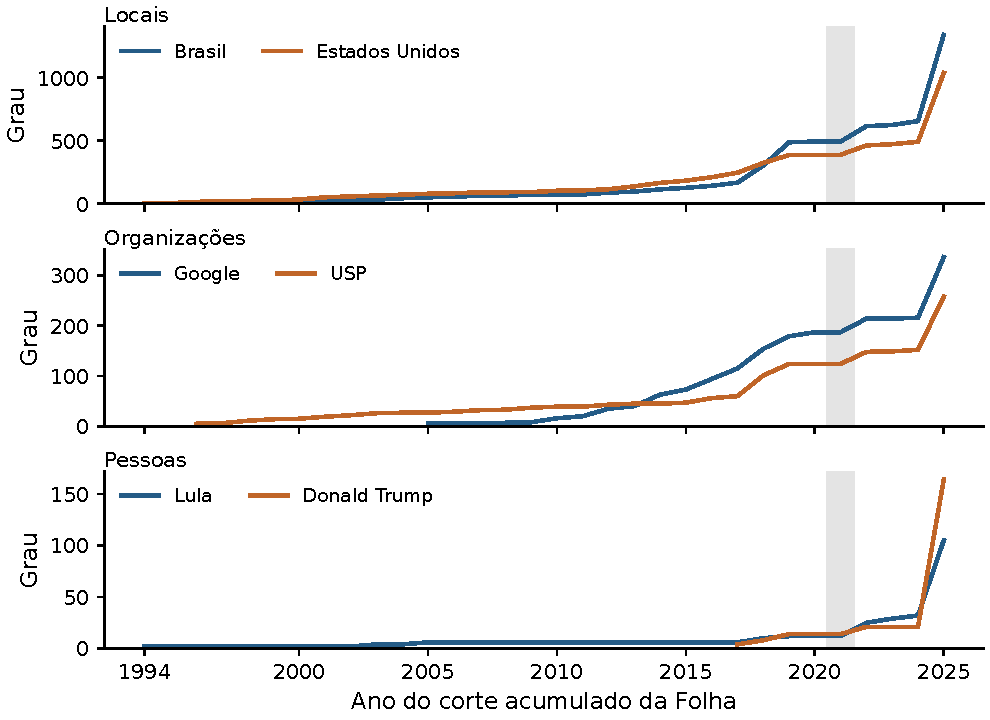
\includegraphics[width=\linewidth,height=12.2cm,keepaspectratio]{figuras/trajetorias_seis.pdf}
\caption{Graus acumulados de seis entidades na Folha, de 1994 a 2025. Os painéis têm escalas verticais próprias. USP corresponde a Universidade de São Paulo; Lula, a Luiz Inácio Lula da Silva. A faixa cinza marca 2021, sem relações acrescentadas por falta de RE. Ausências anteriores à entrada de uma entidade não são preenchidas com zero.}\label{fig:trajetorias}
\end{figure}

Em 2013, Estados Unidos tinha mais vizinhos que Brasil (138 contra 96); em 2019, Brasil já apresentava maior grau (487 contra 386). Entre as organizações, Universidade de São Paulo superava Google em 2013 (45 contra 40), enquanto Google tinha maior grau em 2019 (179 contra 124). Esses contrastes mostram que a ordem observada no corte final não precisa ter sido constante ao longo da série.

Entre as pessoas, Donald Trump passa de grau 21 em 2024 para 164 em 2025, e Lula de 32 para 105. No corte de 2025, Trump aparece em 14º lugar no ranking geral por grau da Folha, e Lula em 28º. Trata-se de posições na rede acumulada, não de medidas de importância política.

Os saltos finais coincidem com a cobertura de RE muito maior em 2025. O grau acumulado também preserva conexões registradas em anos anteriores. Assim, as trajetórias ilustram mudanças de conectividade nos documentos incorporados, sem distinguir, por si, crescimento real de visibilidade e ampliação do processamento.

\clearpage
\section{Distribuição de graus e associação temporal}
\subsection{Cauda e concentração}
A inspeção visual da CCDF foi complementada por ajuste discreto de lei de potência por máxima verossimilhança e seleção de $k_{\min}$ pela distância KS, conforme a abordagem de Clauset, Shalizi e Newman~\cite{clauset2009}. Modelos alternativos são comparados sobre a mesma amostra da cauda. Não foi usada regressão linear sobre coordenadas logarítmicas.

No corte acumulado de 2025, $k_{\min}=2$, $\widehat\alpha=2,4501$ e $D_{KS}=0,004921$. O ajuste abrange 11.435 entidades, ou 41,37\% da rede. Isso delimita a região analisada e impede tratar um ajuste de cauda como descrição uniforme de todos os graus.

\figura{tail}{6.2cm}{CCDF dos graus da Folha acumulada até 2025 e lei de potência ajustada para grau a partir de 2. A curva ajustada é escalada pela proporção de nós da cauda.}

A razão de log-verossimilhança da lei de potência contra a lognormal é $R=-1,3716$, com diagnóstico sob hipótese de observações independentes (iid), $p=0,4665$, sem separação convincente nessa referência. Contra a exponencial, $R=5.201,7210$ favorece a lei de potência, mas preferência relativa não comprova adequação absoluta. A lei de potência com corte é praticamente indistinguível neste ajuste; a comparação é aninhada e requer cautela de calibração.

O bootstrap semiparamétrico de 2025 completou 199 réplicas, com $p=0,20$ e erro Monte Carlo aproximado 0,0284. Trata-se de uma referência iid sobre a distribuição univariada dos graus. Ela não preserva dependências ou restrições topológicas de uma rede. Não rejeitar nessa referência não prova que o mecanismo gerador seja uma lei de potência. Em 2012, o valor final da comparação com a lognormal foi reproduzido com cálculo numericamente estável, mas isso não demonstrou estabilidade dos parâmetros estimados. O alerta permanece, sem preferência conclusiva entre os modelos nesse ano.

Como complemento, o Gini dos graus finais é 0,5339. Os 277 nós do grupo superior de aproximadamente 1\% concentram 24,47\% da soma dos graus. Essa proporção conta extremidades de pares, não a fração de pares exclusivos incidentes no grupo. Concentração e forma da cauda respondem a perguntas distintas. Nesta edição, não se conclui que toda a rede seja livre de escala.

\clearpage
\subsection{Grau anterior e aquisição de novos vizinhos}
A análise temporal pergunta se entidades já presentes com maior grau no corte anterior adquirem mais vizinhos no ano seguinte. Para cada entidade preexistente, considera-se $\Delta k_i(t)=k_i(t)-k_i(t-1)$. Entrantes são examinados separadamente, sem imputar grau anterior zero. Todos os nós anteriores são mantidos, inclusive os sem ganho e os sem notícia observada no ano.

O conjunto analisado contém 133.259 observações de entidades nas transições anuais, das quais 126.880 têm ganho zero (95,21\%). A presença desses zeros é parte do resultado e impede selecionar apenas entidades que cresceram. A correlação de Spearman compara as posições das entidades nos rankings de grau e ganho, considerando os empates; não são usados p-valores que presumam observações independentes. As transições são analisadas separadamente, sem empilhar anos para inferência de observações independentes.

\figura{advantage}{6.5cm}{Associação entre grau anterior e novos vizinhos, acompanhada dos indicadores de cobertura. As curvas descrevem a rede observada; não constituem estimativas causais.}

Nas 30 transições com variação, a associação global entre grau anterior e novos vizinhos é positiva, entre 0,0615 e 0,3096. Em 2024--2025, $\rho_S=0,3096$ entre 14.798 entidades preexistentes, com ganho total de 15.814 extremidades correspondentes a novos vizinhos. O total não equivale ao número de pares novos: cada conexão entre dois nós anteriores incrementa o grau de ambos. Em 2021 não há variação suficiente para calcular a associação; o resultado é ausente, não zero.

As referências uniforme e proporcional ao grau conservam o ganho agregado e servem como comparações algébricas. Não são simulações de grafos nem modelos nulos probabilísticos, não representam saturação das possibilidades de ligação e não fornecem, por si, teste de conexão preferencial. Estratos por tipo, antiguidade e exposição documental são análises descritivas; exposição contemporânea pode participar do próprio mecanismo observado.

A associação positiva é compatível com vantagem cumulativa na rede registrada. Entretanto, diferenças de cobertura, oportunidades de ligação, tipo e exposição podem produzir ou modificar esse padrão. O trabalho não identifica causalidade, não ajusta um expoente de conexão preferencial e não comprova Efeito Mateus sociológico. Persistência, concentração, cauda e associação temporal são evidências complementares, não sinônimos de um mesmo mecanismo.

\clearpage
\section{Discussão e cumprimento dos objetivos}
A análise final desenvolve as três frentes do projeto. A rede global é esparsa e heterogênea, com uma componente dominante. A comparação entre fontes encontra líderes compartilhados, mas baixa coincidência entre os conjuntos de pares. A série da Folha distingue entrada de entidades, formação de conexões, reforço e permanência entre os destaques.

A análise de seis líderes globais e seis casos por tipo mostra que conectividade, recorrência e visibilidade documental são dimensões complementares. Brasil lidera o grau, Estados Unidos a presença em notícias da rede, e Donald Trump combina menos vizinhos que Google com maior visibilidade documental. A concentração das aparições em poucas entidades caracteriza o material observado, sem medir diretamente influência ou destaque editorial.

\begin{table}[H]\centering\small
\caption{Como os resultados atendem aos objetivos apresentados.}\label{tab:objetivos}
\begin{tabularx}{\linewidth}{p{3.8cm}X}\toprule
Objetivo & Resultado e alcance\\\midrule
Geral: comparação e temporalidade & Redes de três fontes comparadas em 2025 e série acumulada da Folha, com a rede global como referência.\\
1. Caracterizar a estrutura & Conectividade, fragmentação, graus, distâncias exatas na GCC e comunidades, com diagnóstico de conectividade interna.\\
2. Comparar fontes & Estrutura, sobreposição de entidades e pares, centralidades e partições, com diferenças de cobertura explicitadas.\\
3. Examinar a evolução & 32 cortes acumulados e separação entre conexões novas e reforço; interpretação limitada nos anos com lacunas.\\
4. Investigar protagonismo e ganhos & Persistência nos rankings, ajustes de cauda, concentração e associação entre grau anterior e novos vizinhos.\\
5. Manter ligação com as notícias & Identificadores e evidências documentais preservados; cobertura usada para contextualizar os resultados.\\\bottomrule
\end{tabularx}\end{table}

Os objetivos foram desenvolvidos dentro do recorte com relações disponíveis, sem equivaler ao processamento integral do acervo. Em relação à entrega parcial, a principal ampliação é passar da descrição inicial da estrutura para a comparação entre fontes e a análise anual da expansão, acrescentando interpretação dos protagonistas e da concentração de visibilidade.

\subsection{Limitações e trabalhos futuros}
A seleção de veículos, a disponibilidade dos textos, os erros de NER/RE e as decisões de identificação das entidades condicionam a rede. A visibilidade mede participação nas relações incorporadas, não todas as menções do corpus. Também permanecem variantes que exigem revisão contextual, como abreviações geográficas e possíveis referências às próprias fontes.

A cobertura de extração varia no tempo. Em especial, 2021 não acrescenta relações; 2020 e 2024 têm baixa cobertura. Essas lacunas impedem interpretar ausência de crescimento como ausência de acontecimentos. A identificação das entidades usa informações do corpus completo, e a acumulação mantém conexões anteriores; o desenho não observa sua dissolução.

\clearpage
As comunidades desconexas em algumas execuções de Leiden foram reproduzidas, mas sua causa permanece aberta. O diagnóstico não justifica modificar automaticamente as partições nem interpretar os grupos como temas validados. O ajuste lognormal de 2012 também conserva uma ressalva sobre a estabilidade dos parâmetros. Dependências entre graus limitam a interpretação dos diagnósticos estatísticos baseados em observações independentes.

Como continuidade, propõe-se concluir a RE dos anos e documentos pendentes, incorporar as extrações adicionais realizadas separadamente e atualizar as redes, tabelas e figuras dependentes. Essas extrações ainda não integram os números desta edição. Também são pertinentes a revisão de identidades e variantes das fontes, a leitura qualitativa de notícias e comunidades e a análise de redes por janelas de tempo, que permitiria distinguir permanência acumulada de presença em cada período. A rede conjunta de 2025 permanece como extensão do planejamento parcial.

\subsection{Conclusão}
O trabalho caracteriza a organização relacional do noticiário sobre IA e mostra como ela varia entre fontes e ao longo do tempo. A estrutura combina baixa conectividade para a maioria das entidades, uma componente dominante e forte desigualdade de presença documental. Entre fontes, um núcleo de protagonistas compartilhados convive com redes de conexões distintas. Na série acumulada, a formação de pares entre entidades novas e antigas representa cerca de metade das novas conexões.

A associação positiva entre grau anterior e aquisição de vizinhos é compatível com vantagem cumulativa na rede observada, mas não identifica um mecanismo causal. A contribuição está em integrar estrutura, comparação, temporalidade e exemplos de entidades, mantendo claras as diferenças entre descrição dos dados e interpretação social.

\subsection{Código e materiais de reprodução}
O código compreende o notebook principal, os módulos de processamento e análise e os scripts complementares. A documentação de execução e as versões correspondentes aos resultados devem acompanhar esses arquivos no repositório:

\noindent\fbox{\parbox{.95\linewidth}{\textbf{Repositório da implementação:} inserir o endereço confirmado antes da entrega.}}

As tabelas de suporte, os scripts da análise complementar e as fontes deste relatório acompanham o pacote de revisão. A documentação técnica conserva parâmetros, verificações e identificação das entradas para permitir a conferência dos resultados.

\begin{thebibliography}{9}\footnotesize\setlength{\itemsep}{1pt}\setlength{\parskip}{0pt}
\bibitem{interian2026mo438} Interian, R. \textit{MO438 -- Redes Complexas: materiais da disciplina}. Instituto de Computação, UNICAMP, 2º semestre de 2026. Disponível em: \url{https://ic.unicamp.br/~ruben/2026/S2-MO438/}. Acesso em: 20 nov. 2026.
\bibitem{godoy2026} Godoy, P. H. C. \textit{Relação IA-sociedade representada na mídia: construção e análise multidisciplinar de redes de entidades nomeadas a partir de textos de notícias}. Dissertação de mestrado, Instituto de Computação, UNICAMP, 2026. Manuscrito fornecido pelo autor.
\bibitem{wang2024e5} Wang, L.; Yang, N.; Huang, X.; Yang, L.; Majumder, R.; Wei, F. \textit{Multilingual E5 Text Embeddings: A Technical Report}. arXiv:2402.05672, 2024. \url{https://arxiv.org/abs/2402.05672}.
\bibitem{blondel2008} Blondel, V. D.; Guillaume, J.-L.; Lambiotte, R.; Lefebvre, E. Fast unfolding of communities in large networks. \textit{Journal of Statistical Mechanics}, P10008, 2008. \href{https://doi.org/10.1088/1742-5468/2008/10/P10008}{doi:10.1088/1742-5468/2008/10/P10008}.
\bibitem{traag2019} Traag, V. A.; Waltman, L.; van Eck, N. J. From Louvain to Leiden: guaranteeing well-connected communities. \textit{Scientific Reports}, 9, 5233, 2019. \href{https://doi.org/10.1038/s41598-019-41695-z}{doi:10.1038/s41598-019-41695-z}.
\bibitem{clauset2009} Clauset, A.; Shalizi, C. R.; Newman, M. E. J. Power-law distributions in empirical data. \textit{SIAM Review}, 51, 661--703, 2009. \href{https://doi.org/10.1137/070710111}{doi:10.1137/070710111}.
\end{thebibliography}
\end{document}
